\documentclass[proseminar,german,utf8]{zihpub}
\usepackage{setspace}
\usepackage{hyperref}
\usepackage{graphicx}
\author{Paul Gottschaldt}
\title{Julia - High-Performance Programmiersprache für High-Performance Computing?}
\matno{4609055}
\betreuer{Martin Schroschk}
\bibfiles{references}
\copyrighterklaerung{Hier soll jeder Autor die von ihm eingeholten
Zustimmungen der Copyright-Besitzer angeben bzw. die in Web Press
Rooms angegebenen generellen Konditionen seiner Text- und
Bild\"ubernahmen zitieren.}
\acknowledgments{Die Danksagung...}

\begin{document}
Das ist eine Referenz auf Klein~\cite{blackholes}. Die Referenzliste ist in der Datei references.bib definiert.
\section {Einleitung}
1998 startete das Apache-Point-Observatorium in New Mexico(USA) ihr Projekt Sloan Digital Sky Survey (SDSS), welches Fotos von über 35~\% aller sichtbaren Objekte unseres Himmels anfertigte und in einer Datenbank zunächst sicherte. Seit diesem Jahr wurden bereits über 500 Millionen Sterne und Galaxien fotografiert und Licht eingefangen, welches bereits Milliarden von Jahren unterwegs war und die Forscher bis weit in die Vergangenheit unseres Universums zurückblicken lässt. Die SDSS-Kamera galt als produktivste Weltraumkamera der Welt bis zu ihrer Abschaltung im November 2009. Mit etwa 200 GB reine Bilddaten pro Nacht entstand so eine Datenbank mit über 5 Millionen Bildern von jeweils 12 Megabyte - zusammengerechnet also rund 55 Terabyte\footnote{\url{https://juliacomputing.com/press/2016/11/28/celeste.html}}. 2014 startete ein Team von Astronomen, Physikern, Informatikern und Statistikern das Projekt Celeste, um eben jenen Datensatz zu katalogisieren und für jeden Himmelskörper einen Eintrag anzulegen\footnote{\url{https://juliacomputing.com/case-studies/celeste.html}}. In der ersten veröffentlichten Version von 2015 noch auf Berechnungen auf einzelne Knoten beschränkt, schaffte es das Forschungsteam um die involvierten Parteien Julia Computing, UC Berkeley, Intel, National Energy Research Scientific Computing Center (NERSC) und Lawrence Berkeley National Laboratory in der zweiten Version von 2016 bereits einen 225-fachen Geschwindigkeitsgewinn zu erzielen. Die größten Verbesserungen waren dabei der mit 8192 Intel® Xeon® Prozessoren ausgestattete Hochleistungsrechner( zu engl. High-Performance-Computer oder HPC) des Berkeley Lab's und \textit{Julia}, eine High-Performance Open-Source Programmiersprache, die bis dato noch relativ unbekannt war und seit 2009 am MIT entwickelt wird. Besonders ist an \textit{Julia} vorallem ihr Anspruch, eine sehr produktive (high-programming language) wie \textit{Python} zu sein, dabei aber Performanz wie \textit{C} zu erreichen. Im November 2017 veröffentlichte dieses Team dann die aktuelle dritte Version, mit der sie nochmals einen deutlichen Geschwindigkeitsgewinn erreichen konnten. Sie schafften es 188 Millionen Sterne und Galaxien in nur 14,6 Minuten zu katalogisieren und nutzten dafür bis zu 1,3 Millionen Threads auf den 9300 Knights Landing(KNL) Knoten des Cori Supercomputers des NERSC. Dabei erzielten sie mit \textit{Julia} eine Peak-Performance von 1.54 PetaFlop/s für Berechnungen mit doppelter Genauigkeit. Damit erzielte das Celeste Projekt einen 100-fachen Performanzgewinn zu allen vorherigen Forschungsprojekten. Derzeit gibt es rund 200 Supercomputer in der Welt, welche in der Lage sind eine Peak-Performance von mehr als einem Petaflop pro Sekunde zu erreichen. Trotzdem sind so gut wie alle Anwendungen, welche eben jene Peak-Performance erreichen von wenigen Gruppen von Experten geschrieben, welche ein sehr tiefes Verständnis für alle erforderlichen Details besitzen, die benötigt werden, um solch eine Performanz zu erreichen\footnote{\url{https://www.nextplatform.com/2017/11/28/julia-language-delivers-petascale-hpc-performance/}}. Umso erstaunlicher ist an diesem Ergebnis also die Tatsache, dass das Team hinter Celeste ihre Geschwindigkeit ausschließlich unter Nutzung ihrer Kenntnisse, dem \textit{Julia}-Code und dessen Threading-Model erzielen konnten.

\begin{figure}[hbt!]
  \centering
  \caption{Eine Abbildungsbeschreibung}
  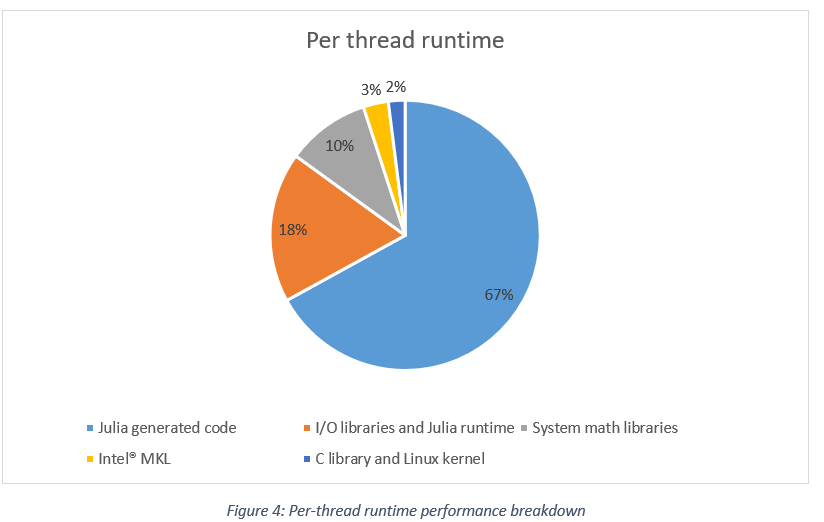
\includegraphics[scale=0.5]{celestejulia.png}
  \label{fig:celestejulia}
\end{figure}

Wie in der Abbildung~\ref{fig:celestejulia} zur pro Thread Auslastung zu sehen, lieferte \textit{Julia} 82.3~\% der Performance. Damit stellt \textit{Julia} unter Beweis das es sowohl für TheraByte-große Datensätze, wie auch für PetaFlop/s-schnelle Berechnungen geeignet ist. Keno Fischer, CTO von Julia Computing, sagte 2017, das Projekte wie Celeste unter Beweis stellen, das der Traum, der hinter \textit{Julia} steht, wahr wird. Wissenschaftler können nun auf ihrem Rechner entwickelte Prototypen einfach von ihrem Laptop auf die größten Supercomputer verschieben ohne zwischen Sprachen wechseln zu müssen oder ihren Code gar komplett neu zu schreiben. Sie (Anmerkung: Entwickler von Julia Computing) sind sehr stolz darauf, dies alles geschafft zu haben und glauben sehr daran, das \textit{Julia} die Entwcklung in der Forschung für viele Jahre sehr voranbringen wird. Viral Shah, CEO von Julia Computing, sagte das Forscher sich nun auf die Lösung ihrer Probleme fokussieren können und sich nicht mehr mit dem Programmieren beschäftigen müssen\footnote{\url{https://juliacomputing.com/press/2016/11/28/celeste.html}}.
%%%%%%%%%%%%%%%%%%%%%%%%%%%%%%%%%%%%%%%%%%%%%%%%%%%%%%%%%%%%%%%%%%%%%%%

\section{Einführung in die Programmiersprache Julia}

\subsection{Übersicht}

\textit{Julia} ist eine junge, flexible, höhere Programmiersprache, die es sich selbst als Ziel gesetzt hat, die hohe Produktivität und einfache Handhabbarkeit aus Sprachen wie \textit{Python} mit der Geschwindigkeit von \textit{C} zu kombinieren. Auch wenn sie vorallem für wisssentschaftliches und numerisches Programmieren gestaltet worden ist, bietet sie eine sogleich performante wie auch einfach zu lernende Umgebung und versucht damit den derzeitigen Trend von mehrsprachigen Softwarelösungen in der Wissenschaft entgegen zu wirken. Mit einem Syntax der an eine Kombination aus \textit{MATLAB} und \textit{Python} erinnert, \textit{Lisp}-ähnlichen Macros und Metaprogrammierung, einem Compiler der \textit{LLVM} nutzt und einem eigenem Paketmanager der an \textit{Git} erinnert, hat sich \textit{Julia} viele bereits etablierte Funktionen zunutze gemacht. Zusätzlich besitzt sie die Möglichkeit \textit{C}- und \textit{Python}-Funktionen einfach direkt aufzurufen, was die Nutzung der Bibliotheken der beiden Sprachen direkt im \textit{Julia}-Code ermöglicht. \textit{Julias} gute Performanz wird vorallem durch Multimethoden für einzelne Funktionen und die automatische Generierung von effizientem typspezialisierten Code gewonnen. Dabei ist \textit{Julia} sowohl dynamisch wie auch statisch typisiert. Zudem ist \textit{Julia} funktional, objektorientiert und imperativ und wurde fast komplett in \textit{Julia} selbst geschrieben.
%%%%%%%%%%%%%%%%%%%%%%%%%%%%%%%%%%%%%%%%%%%%%%%%%%%%%%%%%%%%%%%%%%%%%%%

\subsection{Typensystem und Multimethoden}

In \textit{Julia} gibt es keine Klassen wie es sonst für objektorientierte Sprachen üblich ist. Stattdessen werden in \textit{Julia} Daten eines Objektes explizit von dessen Methoden getrennt. Vom Nutzer angelegte Objekte, wie sie aus anderen puren objektorientierten Sprachen wie \textit{C++} oder \textit{Java} bekannt sind, ähneln am meisten dem \textit{Composite Types}. Auch bekannt unter Namen wie \textit{struct} oder \textit{records} stellt er eine Ansammlung von benannten Feldern da. Diese einzelnen Felder können wie einzelne Attribute betrachtet werden und besitzen einen Wert. Im Sinne der Objektorientierung können die \textit{Composites} ineinander verschachtelt werden. Zusätzlich erzeugt \textit{Julia} standartmäßig für jeden \textit{Composite Type} auch Konstruktoren. Auch wenn \textit{Julia} dynamisch ist und damit der Typ nicht angegeben werden muss, besitzt jeder Wert einen festen Datentyp. Dies gilt auch für die vom Nutzer erstellten Typen. Dabei sind alle Datentypen Laufzeittypen, das heißt den einzigen Datentyp den ein Wert besitzt, ist sein wirklicher aktueller Typ, während das Programm läuft. Auch besitzen nur Werte einen Typ, eine Variable stellt lediglich einen Namen gebunden an einen Datentyp dar. \textit{Julias} Rückgrat für das Typensystem sind die abstrakten Datentypen. Während ein Wert immer einen konkreten Datentyp besitzt, ist dieser Typ gleichzeitig in einen Graphen von abstrakten Typen eingebunden. Konkrete Typen sind die Knoten dieses Graphen und können keine Elternknoten sein. Abstrakte Typen dagegen können mehrere Kinder- und Elternknoten besitzen und bilden die Basis von \textit{Julia}. Der Datentyp \textit{Int64} ist zum Beispiel Kindknoten vom abstrakten Typ \textit{Signed}, welcher Kindknoten vom Typ \textit{Integer} ist. Als oberster Knoten steht der Datentyp \textit{Any}, welcher kein Kindknoten ist. Ein Nutzer kann seine definierten Objekte in diesen Graphen einfügen. Wird nichts weiter spezifiziert, wird das Objekt standartmäßig als Kind vom Typ \textit{Any} angenommen. Als ein weiteres Feature unterstützt \textit{Julia} auch parameterisierte Datentypen. Diese ermöglichen die generische Erstellung von vielen kombinierten Datenypen und dienen zudem unterstützend für \textit{Julias} weiteres Schlüsselmerkmal \-  die Multimethoden. Im Kontext von \textit{Julia} stellen Funktionen ein Objekt dar, welches ein Tuple von Eingangswerten einem Rückgabewert zuordnet oder einen Fehler wirft. Eine einzelne Funktion fasst dabei einen Sachverhalt wie z.~B. die Addition von Werten zusammen und besitzt unterschiedlich viele verschiedene Methoden, welche je nach Anzahl der Argumente und Typ jedes einzelnen Wertes gewählt wird. Deshalb werden Funktionen in \textit{Julia} auch generisch genannt. Methoden widerrum sind nun eine explizite Implementierung einer Funktion und werden nach dem Multimethoden-Verfahren (in Englisch multiple dispatch) ausgewählt. Damit grenzt sich \textit{Julia} im Sinne des objektorientierten Paradigmas sehr von Sprachen wie \textit{Java} oder \textit{C++} ab. Während in diesen Sprachen eine Zuordnung nach dem Typ des ersten Arguments (single dispatch) implizit entschieden wird (zB etwas wie \textit{obj.meth(arg1,arg2)}) werden Methoden in \textit{Julia} explizit nach dem am exaktesten passenden Argumenttypen (z.~B. etwas wie \textit{meth(arg1::Int64,arg2::Number)}) ausgewählt. Am exaktesten passenden Typ meint hier das vom konkreten Typ des Eingabewertes aufsteigend der Typenbaum abgegangen wird, bis eine Methode gefunden wurde, die der Anzahl der Argument und deren Typen entspricht. Wird keine gefunden, so wird ein Fehler geworfen. Multimethoden kombiniert mit den Trennen der Funktionen von den Objekten, auf denen sie arbeiten und dem Typenbaum, ergibt damit eine Art Vererbung die je nach Eingabetypen einer Funktion Verhalten weiterreicht und dabei die Struktur ignoriert. Die Entwickler von \textit{Julia} selbst sagen, das sie festgestellt haben, das die ledigliche Vererbung von Verhalten unter Ausgrenzung der Struktur bestimmte Schwierigkeiten der objektorientierten Sprachen lösen konnte ohne große Nachteile festzustellen. 

Dies ergibt sich daraus, das Mehrfachvererbung auf konkreten Typen zu einer Hierarchie führt, welche sich nicht gut auf die Wirklichkeit mehr abbilden lässt und auch allgemein alles viel mehr verkompliziert wie man zB am Diamant-Problem gut erkennen kann. Julia hat sich explizit dagegen entschieden, in ihr würde jeder konkrete Typ einem seperaten Blattknoten zugeordnet werden und Typen mit ähnlichen Eigenschaften unter einem abstrakten Typ zusammen gefasst werden.
%%%%%%%%%%%%%%%%%%%%%%%%%%%%%%%%%%%%%%%%%%%%%%%%%%%%%%%%%%%%%%%%%%%%%%%

\subsection{Metapr. - eine Hommage an Lisp}

Ein weiteres wichtiges Merkmal von \textit{Julia} ist die Unterstützung für Metaprogrammierung. Wie in \textit{Lisp}, repräsentiert \textit{Julia} seinen eigenen Code als Datenstruktur in sich selbst. Da dieser Code durch Objekte dargestellt wird, kann er genauso aus \textit{Julia} heraus auch erstellt und manipuliert werden. Dadurch wird es möglich Code zu transformieren oder gar Code zu generieren. \textit{Julia} repräsentiert zudem alle Datentypen und den Code in Strukturen, welche in \textit{Julia} implementiert worden sind, wodurch auch eine sehr mächtige Rückschau (engl. Reflection) möglich ist. Ein Ausdruck wird dabei immer in ein \textit{Expr} - Objekt übersetzt, welches sowohl den Typ des Ausdrucks wie auch seine Argumente beinhaltet und in \textit{Julia} sehr einfach zu bearbeiten oder auszuwerten ist. Dem Datentyp \textit{Symbol} wird hierbei noch eine sehr bedeutende Rolle zugedacht. Er repräsentiert alle Variablen und damit verbunden auch Zuweisungen und Funktionsaufrufe. Damit ist es möglich Daten von einer Variablen auch in der Datenstruktur noch zu unterscheiden. \textit{Julia} besitzt auch \textit{Lisp}-ähnliche Macros. Dies sind Funktionen, welche einen Ausdruck als Argument nehmen, ihn manipulieren oder zusätzlichen Code hinzufügen und dann eine Ausdruck zurückgeben. Der Unterschied zu herkömmlichen Funktionen ist vorallem der Zeitpunkt zu dem ein Macro ausgewertet wird. Es wird ausgeführt wenn der Code übersetzt wird und bietet damit die ideale Möglichkeit Funktionen zusätzlich zu manipulieren. Ein gängiges später noch sichtbares Beispiel wäre hier das @\textit{Benchmark} Macro welches Performanztests ausführt und am Ende neben dem Ergebnis auch die Laufzeit, die Allokationen und den benötigten Speicher für die Funktion zurückgibt. Um die Erstellung und Manipulation von Ausdrücken zu vereinfachen gibt es zudem die Funktion, eine Variable in den Ausdruck im Nachhinein einzufügen. Dieses Verfahren nennt sich zu englisch \textit{splicing} oder \textit{interpolating}. Da so auch lokale Variablen in Macros übergeben werden können ist es für diese sehr nützlich, da normal übergebene lokale Variablen sonst innerhalb des Macros undefiniert sind um das versehentliche Übernehmen oder Überschreiben von Variablen im inneren Anwendungsbereich (scope) zu verhindern.
%%%%%%%%%%%%%%%%%%%%%%%%%%%%%%%%%%%%%%%%%%%%%%%%%%%%%%%%%%%%%%%%%%%%%%%

\subsection{JIT Compiler auf Basis von LLVM}

\textit{Julias} Compilierungsprozess beginnt mit der Definition einer Methode und deren Ausführung. Auch wenn \textit{Julia} dynamisch ist, so ist sie dennoch stark typisiert und macht sich den Low Level Virtual Machine (\textit{LLVM}) Echtzeit (just in Time oder JIT) Compiler zu nutze, um nativen Maschinencode zur Laufzeit zu generien. Dabei besteht dieser Prozess der Generierung aus vier Stufen und für jede Stufe bietet \textit{Julia} eigene Funktionen um sich den generierten Code ausgegeben zu lassen. In der ersten Phase, der sogenannten niedriger Code (\textit{code\_lowered}) Phase wird der Code etwas vereinfacht und gleichzeitig deutlich ausdrucksstärker gemacht um dem Compiler die nächsten Schritte deutlich zu vereinfachen. An dieser Stelle werden auch generische Funktionen eingebunden, welche für unterschiedliche Argumente unterschiedlichen niedrigeren Code erzeugen. In der nächsten Stufe wird versucht über alle Typen die im Code vorkommen eine Schlussfolgerung zu schließen und lokale Optimierungen basierend auf den ermittelten Typen zu treffen. In der dritten Phase wird dieser, an die Typen angepasste Code, dann mit dem \textit{LLVM}-JIT-Compiler zu \textit{LLVM}-Code übersetzt  und schlussendlich in der vierten Stufe zu nativen Maschinencode herunter compiliert. Dieser Maschinencode wird dann zwischengespeichert und erneut ausgeführt, sobald die Funktion erneut mit gleichen Argumenttypen und der gleichen Anzahl an Argumenten aufgerufen wird, wodurch sich die zeitintensive JIT- Phase ersparen lässt und eine Funktion bei erneuter Ausführung mit gleichen Parametern sehr viel schneller läuft.
%%%%%%%%%%%%%%%%%%%%%%%%%%%%%%%%%%%%%%%%%%%%%%%%%%%%%%%%%%%%%%%%%%%%%%%

\subsection{Interne und externe Bibliotheken}

Auch wenn \textit{Julia} noch eine sehr junge Sprache ist, bietet sie bereits jetzt eine sehr schnell wachsende Sammlung an verschiedensten Paketen, die verschiedenste Funktionen bereitstellen und sich einfach über \textit{Julias} eingebauten Paketmanager verwalten lassen. Dieser installiert, deinstalliert und aktualisiert die Pakete deklarativ, das heißt er findet selbst heraus welche Versionen noch benötigt werden oder welche veraltet sind und gelöscht werden können. Intern nutzt der Manager das \textit{libgit2} Framework und setzt damit direkt auf \textit{git} auf. Alle Pakete sind dabei einfache \textit{git} Repositories und klonbar, wie es von \textit{git} bekannt ist. Die Pakete müssen dabei einer gewissen Format-Konvention folgen und im \textit{Metadata.jl} Repository registriert sein, damit \textit{Julia} das Paket finden kann, unter der Angabe der URL für unregistrierte Pakete gibt es aber eine Möglichkeit für diese, eingebunden zu werden. Zudem wird \textit{Julias} Paketmanager derzeit sehr umfangreich überarbeitet und es ist zu erwarten, das in der nächsten Version 0.7 \textit{Julias} Paketverwalter um eine Funktionen erweitert und verbessert wird. Neben diesem Paketmanager für eigene \textit{Julia}-Pakete bietet die Sprache aber auch eine sehr einfache Maske um \textit{C}- oder \textit{Fortran}-Funktionen und Werte direkt aus \textit{Julia} aufzurufen und stellt damit ideale Möglichkeiten zur Integration in einer bereits etablierten Umgebung zur Verfügung. Dabei funktioniert alles ganz ohne Klebstoff-Code mit einem einfachen Funktionsaufruf wie z.~B. \textit{ccall()} und da der von \textit{Julias} JIT native generierte Code am Ende der Gleiche wie der native \textit{C} Code ist, gibt es keinen Verlust bei der Performanz. Auch \textit{Python} oder \textit{C++} über ein Paket lassen sich sehr einfach einbinden, zudem gibt es noch die Möglichkeit aus Julia heraus direkt externe Programme aufzurufen.
%%%%%%%%%%%%%%%%%%%%%%%%%%%%%%%%%%%%%%%%%%%%%%%%%%%%%%%%%%%%%%%%%%%%%%%

\section{Parallele Programmierung mit Julia}

Als Sprache, die parallele Programmierung als eine ihrer Kernkompetenzen sieht und sich sehr auf Performanz orientiert, wundert es nicht, das \textit{Julia} auch sehr viele Möglichkeiten bietet, um Berechnungen zu parallelisieren.\textit{Julia} hat in diesem Feld eine Fülle von sehr viele einfachen Funktionen für simple Probleme, aber gleichzeitig auch eine Tiefe der Funktionen, um das letzte bisschen Performanz noch rauszukitzeln. Als Grundbaustein für \textit{Julias} Multiprozessorhandhabung dient dabei eine eigene Implementierung einer Nachrichtenübertragung zur Kommunikation zwischen den Prozessen, um diese parallel in seperaten Speicherbereichen laufen zu lassen. Diese Übertragung ist anders als bestehende Konzepte wie MPI und ist so ausgerichtet, das generell nur 1 Seite programmiert werden muss um eine Kommunikation aufzubauen und zu beenden und zusätzlich auch eher wie ein Funktionsaufruf aussieht. In Julia besitzt jeder Prozessoren eine eindeutige Kennzeichnung. Sie macht sich zudem das \textit{Master-Worker} Prinzip zunutze und ernennt den Hauptprozessor zum \textit{Master}-Prozessor mit der Id 1. Solange es mehr Prozessoren als einen gibt, ist der Hauptprozess mit der Id gleich eins immer der \textit{Master}, ansonsten wird er allein als \textit{Worker} angenommen. Dadurch ergibt sich auch, dass das hinzufügen nur eines weiteren Prozessors kaum Performanzgewinn erzielen kann, da der Meisterprozessor bei parallelen Aufgaben nur verwaltet und selber nicht berechnet, außer man weist ihn dazu explizit an. Intialisiert werden können weitere Prozessoren zum einen lokal beim Starten einer \textit{Julia}-Instanz mit dem Attributen \textit{julia -p n}, wo bei \textit{n} für die Anzahl der \textit{Worker} steht, oder aber mit der Funktion \textit{addprocs(n)} sowohl lokal, wie auch remote, wobei hier auch zu der externen Machine via \textit{ssh} eine Verbindung aufgebaut werden muss. Mit der Funktion \textit{workers()} oder \textit{nworkers()} wird ein Array mit den Ids der eingebundenen Arbeiter beziehungsweise die Anzahl der Arbeiter zurückgegeben. \textit{rmprocs(id)} entfernt hingegen nur den \textit{Worker} mit der spezifizierten Id.
%%%%%%%%%%%%%%%%%%%%%%%%%%%%%%%%%%%%%%%%%%%%%%%%%%%%%%%%%%%%%%%%%%%%%%%

\subsection{Remote-Aufrufe und -Referenzen}

\textit{Julias} parallele Programmierung ist auf zwei primitiven Objekten aufgebaut: Remote-Referenzen und Remote-Aufrufe. Eine Remote-Referenz ist eine Instanz, die von jedem Prozessor aus genutzt werden kann und auf ein auf einem bestimmten Prozessor gespeicherten Objekt zeigt. Ein Remote-Aufruf ist ein Antrag von einem Prozessor eine bestimmte Funktion mit bestimmten Argumenten auf einem Prozessor, der auch der gleiche wie der aufrufende sein kann, auszuführen. Remote-Referenzen gibt es in der Ausprägung \textit{Future} und als einen \textit{RemoteChannel}. Ein \textit{Future} ist der Rückgabewert eines Remote-Aufrufs, der direkt zurückgegeben wird, um den Prozess während seiner Ausführung nicht zu blockieren. Dieser kann dan mittels eines \textit{fetch()} geholt werden, sobald das Ergebnis vorliegt. Ein wichtiger Hinweis ist hier zudem, das ein einmal mit \textit{fetch()} geholtes \textit{Future} lokal gespeichert wird und deshalb bei einem erneuten \textit{fetch()} keine weitere Kommunikation anfällt. \textit{RemoteChannel} wiederum sind wiederbeschreibare Kanäle, die auch als Überbrücker zwischen Kanälen (Channel) verstanden werden können. Ein Kanal ist dabei eine Leitung zwischen Prozessen (Tasks) oder eben aber auch Prozessoren die genutzt werden um Daten auszutauschen, wobei jeweils immer einer Daten auf den Kanal legt und einer diese Daten abgreift, sobald sie verfügbar sind via \textit{put!()} und \textit{take!()}. Ein Kanal kann dabei immer mehrere schreibende wie auch mehrere lesende Prozesse haben. Ein \textit{RemoteChannel} nimmt hier nun den Aus- oder Eingang eines Kanals auf einem vorher spezifizierten Prozessor und schickt dann die Daten weiter. \textit{Julia} bietet auch zwei Funktionen an um eine Remote-Aufruf direkt auszulösen, normalerweise sind dies aber eher tiefer liegende Funktionen welche der Nutzer nicht selber benutzen muss, sondern die generiert werden durch höhere Funktionsaufrufe. \textit{Remotecall(f,id,args..)} gibt dabei direkt ein \textit{Future} zurück, während \textit{remotecall\_fetch(f,id,args...)} auf den Rückgabewert wartet und darauf dann direkt noch wie der Name es suggiert ein \textit{Fetch} ausführt.
%%%%%%%%%%%%%%%%%%%%%%%%%%%%%%%%%%%%%%%%%%%%%%%%%%%%%%%%%%%%%%%%%%%%%%%

\subsection{@Spawnat und @Spawn}

\textit{Julia} bietet neben dem Remote-Aufruf auch noch zwei weitere Macros an um einen direkten Aufruf an einen anderen Prozessor zu starten und dafür ein \textit{Future}-Referenz zu bekommen. Das \textit{Spawnat} Macro akzeptiert hierbei zwei Argumente pid und expr. Es berechnet den Ausdruck des zweiten Arguments auf dem Prozessor spezifiziert mit dem ersten Argument.  Damit verhält sich das \textit{Spawnat} Macro sehr ähnlich zu einem \textit{remotecall()}, arbeitet dabei jedoch mit einem Ausdruck statt mit einer Funktion. Um diesen Sachverhalt noch zu vereinfachen bietet \textit{Julia} außerdem das @\textit{Spawn} Macro an. Dieses sucht selbständig nach einem unbeschäftigten Prozessor und lagert die Berechnung der Funktion an diesen aus. Dabei verhält sich \textit{Spawn} auch intelligent und erkennt, wenn Werte vorher auf einem bestimmten Prozessor ausgerechnet worden waren, und lagert die darauf aufbauende Berechnung auf eben jenen Prozessor erneut aus um sich den sonst nötigen Fetch zu ersparen. Wichtig zu beachten bei einem Remote-Aufruf ist, das die aufzurufenden Funktionen dem Prozessor bekannt sind, der sie ausführen soll, gleiches gilt auch für geladene Pakete und deren Funktionen und Variablen. Mit dem Macro @\textit{everywhere} kann eine Funktion direkt auf allen Prozessoren definiert werden um dieses Problem zu umgehen. Auch sollte beim Umgang mit einem direkten Remote-Aufruf vorsichtig mit lokalen Variablen umgegangen werden, um einen unnötigen Kommunikationsaufwand zu vermeiden. So würde \textit{julia> message = "This string is constructed locally";
julia> shouting\_message = @spawn uppercase(message)} das Kopieren der Nachricht vom \textit{Master}-Prozessor auf den berechnenden Prozessor erfordern und deutlich mehr Zeit kosten als die lokale Variable direkt im @\textit{spawn} Befehl zu definieren mit \textit{julia> shouting\_message = @spawn uppercase("This string is not constructed locally")}. Aufgepasst werden sollte zudem bei globalen Variablen, da diese nicht synchronisiert werden und sich nicht durch Berechnungen auf anderen Prozessoren beeinflussen lassen.
%%%%%%%%%%%%%%%%%%%%%%%%%%%%%%%%%%%%%%%%%%%%%%%%%%%%%%%%%%%%%%%%%%%%%%%

\subsection{Parallele Map und For-Schleife }

Der obere Teil der parallelen Programmierung war eine kurze Einführung in \textit{Julias} Handhabung von parallelen Berechnungen im Hintergrund. Aber nur in den seltensten Fällen wird ein Entwickler in \textit{Julia} wirklich in die Lage kommen, in denen er manuell eine Berechnung auslagert. Stattdessen bietet \textit{Julia} zwei Funktionalitäten an um Probleme sehr einfach und gut lesbar zu parallelisieren. Die erste Variante umfasst hierbei das Macro @\textit{parallel}, eine parallele For-Schleife, welche besonders optimiert ist für Probleme mit vielen voneinander unabhängieng Iterationen. Dabei ist diese For-Schleife gleichzeitig auch noch eine Reduktionsfunktion und bietet die Möglichkeit, eine Funktion mit zu übergeben, welche am Ende über allen Resultaten ausgeführt wird und dabei die Dimension des Problems um eins reduziert (auch als \textit{tensor-rank-reducing} bekannt). Diese Form ist aber optional und eine parallele For-Schleife funktioniert auch ohne diese übergebene Funktion und gibt für diesen Fall einfach das Ergebnis zurück. Die Berechnung, wie häufig Kopf(n) bei M Münzwürfen auftrat, lässt sich als Beispiel sehr einfach mit @\textit{parallel} Parallelisieren und nutzt zudem die Addition als Reduktion \textit{julia> nheads = @parallel (+) for i = 1:M; Int(rand(Bool));end}. Wichtig zu beachten ist hierbei das, auch wenn sie einer normalen For-Schleife sehr ähnlich sieht, sich eine parallele For-Schleife anders verhält und die Iterationen nicht in Reihenfolge ablaufen und auch globale Variablen sich so nicht beschreibbar lassen. Ein weiterer wichtiger Hinweis an dieser Stelle ist, das der Rückgabewert einer solchen parallelen For-Schleife ohne Reduktionsfunktion ein Array von \textit{Future}'s ist und die Funktion ohne ein \textit{fetch()} direkt weiter läuft, auch wenn noch kein Ergebnis bereit liegen am Ende der Schleife. Hilfreich hierfür ist das Macro @\textit{sync}, welches vor das Macro @\textit{parallel} geschrieben wird um den Prozess zu blockieren, solange wie alle Berechnungen parallel ausgeführt werden. Als zweites Werkzeug stellt Julia eine parallele Map bereit, welche besonders nützlich für große Funktionen, die einzeln auf eine Menge von Elementen angewandt werden muss, ist. \textit{pmap(i-> log(i), 1:M, batch\_size)} berechnet zum Beispiel den Logarithmus der Zahlen eins bis M und speichert sie erneut in einem Array ab. Da \textit{pmap} vorallem für größere Funktionsaufrufe gestaltet worden ist, kann es hier teils extreme Performanzeinbuse bei dem Aufruf von kleinen Berechnungsfunktionen wie\textit{ log()} geben, da der Kommunikationsaufwand sehr groß ist, wenn jeder Wert einzeln auf einem neuen Prozessor berechnet wird und dafür jeweils immer der Wert hin und her kopiert wird. Eine Lösung bietet die Funktion dafür aber direkt selber. Mit dem Attribut \textit{batch\_size} kann die zu kopierende Datengröße festgelegt wird pro Funktionsaufruf an einen anderen Prozessoren festgelegt werden. Die Nutzung von @\textit{parallel}, das für kleine Iterationen optimiert ist, wäre hier aber genauso möglich.
%%%%%%%%%%%%%%%%%%%%%%%%%%%%%%%%%%%%%%%%%%%%%%%%%%%%%%%%%%%%%%%%%%%%%%%

\subsection{Shared und Distributed Arrays}

\textit{Shared Arrays} nutzen gemeinsam genutzten Speicher im System um das gleiche Array über viele Prozessoren hinweg zu verlinken. Im Gegensatz zu einem \textit{Distributed Array}, in dem jeder Prozess seinen eigenen lokalen Zugang zu einem eigenen Teil (\textit{chunk}) des gesamten Arrays besitzt, hat jeder teilnehmende Prozess bei einem \textit{Shared Array} Zugang zum gesamten Feld. Während \textit{Distributed Arrays} vorallem für sehr große Felder, welche zu groß zum Rechnen auf einem einzelnen Prozessor sind, geeignet sind und bei diesen jeder Prozess seinen Teil der Daten verarbeitet, eignen sich \textit{Shared Arrays} besonders für gemeinsames Rechnen, in dem darüber der Kommunikationsaufwand deutlich reduziert wird und zum Beispiel auch Iterationen über globale Arrays mit der parallelen For-Schleife möglich werden. Mit den Funktionen \textit{sdata()} sowie \textit{convert()} und \textit{localpart()} für \textit{Distributed Arrays} lassen sich beide Arrays ganz einfach zu normalen Standartfeldern konvertieren bzw den lokalen Anteil des\textit{ Distributed Arrays} in ein normales Array extrahieren. 
%%%%%%%%%%%%%%%%%%%%%%%%%%%%%%%%%%%%%%%%%%%%%%%%%%%%%%%%%%%%%%%%%%%%%%%

\subsection{vertiefende Themen zum parallelen Programmieren}

Neben diesen doch recht einfachen anwendbaren Funktionalitäten bietet Julia auch noch eine Reihe weitere Möglichkeiten zusätzlichen Performanzgewinn zu erzielen. Die erste Möglichkeit ist dabei die manuelle Handhabung der Lebenszeit der Objekte. Auch wenn der implementierte Müllsammler (Garbage collector) selbst mit der Zeit Objekte aufräumt, so sollte gerade bei Codezeilen mit sehr vielen kleinen und auch kurzlebigen Objekten explizit die Funktion finalize() aufgerufen werden, um lokale Instanzen oder auch Remote-Referenzen oder Shared Array aus dem Speicher zu löschen, da der Remote-Knoten sehr groß sein kann und zudem gerade größere Objekte zuerst vom Garbage Collector gelöscht werden. Ein Löschen des mit fetch() geladenen Future's ist nicht notwendig, da fetch() bereits den Remote-Knoten entfernt. Eine weitere Möglichkeit bietet die eigene Konfiguration eines Clustermanagers. Dieser ist verantwortlich für das Starten der Arbeiter, das Verwalten von Events, die auf den Arbeitern auftreten, und auch für den Datentransport und der Kommunikation zwischen den Prozessoren. Dabei kann beispielsweise vom standartmäßigen TCP/IP hin zu MPI abgewichen oder verschiedene Aufgaben-Warteschlangen wie Slum oder PBS realisiert werden um eine effizientere Auslastung der Prozessoren zu erreichen. Auch stellt Julia mit dem Macro @simd die Option, dem Compiler explizit mitzuteilen, an bestimmten Stellen zu Vektorisieren. Zusätzlich gibt es auch noch verschiedenste Pakete wie zB das ParallelAccelerator-Paket von Intel welches mit dem @acc Macro ein Mittel bietet, bestimmte Teile wie in diesem Fall ressourcenkostende Arrayfunktionen noch einmal deutlich zu beschleunigen. Daneben gibt es auch noch experimentielle Möglichkeiten, welche sich derzeit noch in Entwicklung befinden, aber bereits eingeschränkt nutzbar sind. So lässt sich die Netzwerktopologie des Clusternetzwerkes in die Funktion addprocs() als Argument mitgeben um zu spezifizieren, wie der Arbeiter zu den anderen Prozessoren verbunden werden soll. Auch gibt es bereits erste Möglichkeiten für Multithreading in Julia, wobei hier vorher noch eine Umgebungsvariable außerhalb von Julia gesetzt werden muss um festzulegen, wieviele Threads gestartet werden sollen. Mit dem Macro Threads.@threads lassen sich dann Schleifen Parallelisieren, ähnlich zur @parallel-Variante nur ohne Reduktionsfunktion.
%%%%%%%%%%%%%%%%%%%%%%%%%%%%%%%%%%%%%%%%%%%%%%%%%%%%%%%%%%%%%%%%%%%%%%%

\subsection{Softwarewerkzeuge}

Um das Erlernen der Sprache Julia zu erleichtern oder auch um einfach Fehler und schlecht funktionierende Codezeilen aufzuzeigen, gibt es bereits einige sehr praktische Werkzeuge für Julia. BenchmarkTools zum Beispiel ist ein Paket, welches geschrieben wurde, um mathematisch korrekte Maßstabanalysen (Benchmarks) zu gewährleisten. Neben der Möglichkeit bestimmte Handlungen, wie das Erzeugen von Zufallszahlen auszuklammern, um den Test aussagekräftiger zu gestalten, bietet es zudem verschiedenste Macros und Funktionen an, um die Allokationen, den Speicherverbrauch und auch die Laufzeit der Funktionen zu messen und gibt dabei sogar Minimale, Maximale und Durchschnittswerte zurück. Ein weiteres sehr hilfreiches Werkzeug sind Julias eigenen Macros @code\_native, @code\_typed, @code\_llvm und vorallem @code\_warntype welche den herunter compilierten Code für die entspreche Funktion in dem gewählten Level zurück geben und damit unerwartetes Verhalten gut aufzeigen können. Code\_warntype hebt dabei sogar alle ungenauen Typ-Spezifikationen farblich hervor und eignet sich damit ideal um zu überprüfen, ob jede Variable den günstigsten Typ zugewiesen bekommen hat, denn auch wenn Julia dynamisch ist und Typen nicht explizit genannt werden müssen, kann man so den Code deutlich beschleunigen, da Checks entfallen oder Berechnungen aufgrund gewisser Typinformationen deutlich vereinfacht werden können. Ein weiteres Instrument bietet Julia hier auch noch mit dem Profiling, welches ermittelt, wieviel Zeit pro indivdueller Zeile benötigt worden ist. Auch gibt es einen Linter, welcher Hinweise zum Code gibt und damit aufzeigt, wenn einfachere Implementierungen möglich sind. Ein kurzen Hinweis an dieser Stelle noch bezüglich eines Debuggers, den Julia zwar besitzt, der in seiner derzeitigen Implementierung aber keine Breakpoints oder nativer Code Untersuchung unterstützt und damit bisweilen doch noch etwas ungewohnt zu bedienen ist.
%%%%%%%%%%%%%%%%%%%%%%%%%%%%%%%%%%%%%%%%%%%%%%%%%%%%%%%%%%%%%%%%%%%%%%%

\section{Bewertung der HPC-Eignung von Julia}
\section{Schlusswort}
\end{document}
